\documentclass{article}
\input{../../preambule}

\hypersetup{colorlinks=true, urlcolor=bleu, linkcolor=red}

%Def = Definition
%Theo = Théorème
%Prop = Propriété
%Coro = Corollaire
%Lem = Lemme

\makeatletter
\@addtoreset{section}{part}
\makeatother

\newcommand{\Inde}{\perp \! \! \! \perp}

\begin{document}

\setcounter{tocdepth}{4}
\tableofcontents
\newpage

\part{\'El\'ements finis}
\textit{Problème modèle :} On va considérer une EDP elliptique (basée sur le laplacien $\Delta$, somme des dérivées secondes)
\[(P)\left\{\begin{array}{c c c}
-u''(x) &=& f(x) \\
u(0)&=&u(1)=0
\end{array}\right.\ \forall x\in\Omega=]0,1[  \]

\section{Formulation variationnelle}
Cette formulation permet de "baisser" l'ordre de dérivation (via la formule de Stroke ou une IPP).
\subsection{Choix de l'espace}
On va définir l'espace V :
\[V=\{u\in L^2(\Omega),\ u'\in L^2(\Omega),\ \underbrace{u(0)=u(1)=0}_{\text{Conditions de Dirichlet}}\}\]

\underline{Remarque :} On a intégré les conditions de Dirichlet homogènes dans la définition de V.

\bigskip
On notera $V=H_0^1(\Omega)$ un espace de Sobolev, qui est un espace de Hilbert.\\
On définit :
\[\langle u,v\rangle=\int_{\Omega}uv dX + \int_{\Omega} u'v'dX\]
\[\|v\|^2=\langle v,v\rangle = \|v\|^2_{L^2(\Omega)} + \|v'\|^2_{L^2(\Omega)}\]

\subsection{Recherche de solution}
On cherche la solution $u(x)$ dans V. $\forall v\in V$ (appelée fonction test) :
\begin{eqnarray*}
	-u''=f \\
	-vu''=vf \\
	-\int_{\Omega} u''v dx = \int_{\Omega} fv dx
\end{eqnarray*}

On a de plus :
\[-\underbrace{[u'v]_0^1}_{=0 \text{ car } v\in V} + \int_0^1 u'v' dx = \int_{\Omega} fv dx\]

On se ramène donc au problème suivant ; trouver $u\in V$; $\forall v\in V$ :
\[(P.V.) \left\{ \begin{array}{c c}
a(u,v)=L(v)\\
\text{avec } & a(u,v)=\int_0^1 u'v' x \\
	     & 	L(v)=\int_0^1 fv dx
\end{array}\right.\]

La solution de PV est appelée solution faible \\
La solution de P est appelée solution forte.

\subsection{Existence-unicité d'une solution de (PV)}

\Theo{de Lax-Milgram}{$a(\bullet,\bullet)$ est :
\begin{itemize}
	\item une forme bilinéaire (symétrique ?)
	\item V-elliptique : $a(u,u)\geq \alpha \|u\|_v^2,\ \alpha\geq 0$
	\item continue : $|a(u,v)| \leq C\|u\|_V\|v\|_V,\ C\geq 0$
\end{itemize}
$L(\bullet)$ est linéaire continue.\\
Sous ces conditions, (PV) admet une solution unique $u\in V$.}

\section{Approximation numérique du problème variationnel}
C'est dans cette partie que l'on va utiliser la méthode des élements finis en exprimant la solution discrétisée $u_h$ dans une base d'un espace $V_h$ de dimension finie.

\subsection{Choix de $V_h$}
Choix le plus simple :
\[V_h=\{v_n\in V; v_h\in\mathcal{C}^0(\bar\Omega), \forall i=0,...,n-1;\ {v_h}_{[\tau_i,\tau_{i+1}]}\in\mathbb{R}_1[X]\}\]

$V_h$ est un espace vectoriel de dimension $n-1$. 

\bigskip
\underline{Remarque :} Cela correspond à des $\beta$-splines.
\[\tau=(\tau_i)_{i=0..n},\ \dim \mathbb{P}_{k,\tau,r}=(k+1)n-\sum_{i=1}^{n-1} r_i\]
$\mathbb{P}_{k,\tau,r}$ est l'espace des fonctions polynomiales par morceaux de degré inférieur ou égal à k avec un raccord $\mathcal{C}^{r_i-1}$ en $\tau_i$.

\bigskip
En particulier, $\dim V_h=n-1$.

\subsection{Fonctions de base}
Ce sont les $(\phi_i)_{i=1,...,n-1}$, ils vérifient une condition lagrangienne :
\[\left\{\begin{array}{c c c c}
\phi_i(z_i)&=&1 & \\
\phi_i(z_j)&=&0\ & \forall j\neq i
\end{array}\right.\]

\subsection{Problème discrétisé}
Le problème discrétisé $(PV_h)$ est maintenant la recherche de $u_h(x)=\sum_{j=1}^{n-1} \xi_i \phi_i(x)\in V_h$ tel que $\forall v_h\in V_h, a(u_n,v_n)=L(v_n)$.

\subsection{Détermination des inconnues $(\xi_j)_{j=1,...,n-1}$}
On a :
\[u_h(\tau_i)=\sum_{j=1}^{n-1} \xi_j \phi_j(\tau_i)=\xi_i\]
$(PV_h)$ est équivalent à : \\
Trouver $u_h(x)=\sum_{j=1}^{n-1}\xi_j \phi_j(x)\in V_h$ tel que $\forall i=1,...,n-1$, $a(u_h,\phi_i)=L(\phi_i)$. 

On a fonc:
\[\sum_{j=1}^{n-1} \xi_j \underbrace{a(\phi_j,\phi_i)}_{\text{Matrices de rigidité}}=L(\phi_i),\ \forall i=1,...,n-1\]

On se ramène donc à un système linéaire :
\[R\xi=F\]

\Prop{}{R est définie positive.}

\begin{dem}
On l'obtient grâce à la V-ellipticité de $a(\bullet,\bullet)$. \\
Soit $v\in\mathbb{R}^{n+1}$. On cherche à voir si $v^TRv>0$.

\[(v^TR)_j=\sum_{i=1}^{n-1} v_iR_{ij}=\sum_{i=1}^{n-1} v_ia(\phi_j,\phi_i)=a(\phi_j,\sum_{i=1}^{n-1} v_i\phi_i)\]
\[(v^TR)v=\sum_{j=1}^n v_j(v^TR)_j = a\left( \sum_j v_j\phi_j, \sum_i v_i\phi_i\right)\]

Posons $w=\sum_i v_i\phi_i$, $a(w,w)\geq 0$ car $a(\bullet,\bullet)$ V elliptique. 
\end{dem}

\part{Petits rappels d'analyse fonctionnelle}
\section{Rappels sur les distributions}
\underline{Notation :} $\alpha=(\alpha_1,...,\alpha_n)\in\mathbb{N}^*$, on définit :
\[\partial^\alpha=\frac{\partial^{|\alpha|}}{\partial^{\alpha_1}x_1...\partial^{\alpha_n}x_n}\]
avec $|\alpha|=\sum_{i=1}^n \alpha_i$

\Prop{}{\begin{itemize}
\item $\mathcal{D}(\Omega)$ est dense dans $L^2(\Omega)$ (toute fonction de $L^2(\Omega)$ est limite d'une suite de fonctions incluse dans $\mathcal{D}(\Omega))$.
\item L'application identité de $L^2(\Omega)$ dans $\mathcal{D}'(\Omega)$ est appelée injection canonique. Elle est continue.
\item $f_n\xrightarrow{L^2(\Omega)} f \Rightarrow T_{f_n} \xrightarrow{\mathcal{D}'(\Omega)} T_f$
\end{itemize}}

\section{Espaces de Sobolev}
Ces espaces nous permettent de résoudre les problèmes variationnels. Les espaces de Sobolev se construisent à partir des espaces $L^p$ (on va d'abord s'intéresser aux espaces $H^m(\Omega)$ construits sur $L^2(\Omega)$).

\subsection{Liens entre $\mathcal{D}(\omega)$, $L^2(\Omega)$ et $H^1(\Omega)$}
On rappelle la notion de dérivation faible :
	\[u\in L^2(\Omega),\ \frac{\partial u}{\partial x_i} \to \omega_i \in \mathcal{D}'(\Omega)\]
\Def{Espaces des Sobolev}{Les dérivées qui vont intervenir dans les espaces de Sobolev sont prises au sens des distributions. 
	\[H^1(\Omega)=\left\{v\in L^2(\Omega),\ \frac{\partial v}{\partial x_i}\in L^2(\Omega),\ \forall i=1,...,n\right\}\]
où $\Omega\subset\mathbb{R}^n$. \\
On définit un produit scalaire :
\begin{eqnarray*}
	((u,v))_{1,\Omega}&=&\int_{\Omega} \left(uv+\sum_{i=1}^n \frac{\partial u}{\partial x_i} \frac{\partial v}{\partial x_i}\right) dx\\
			&=&\int_{\Omega} \left( uv + \left(\nabla u\right)^t \nabla v\right) dx
\end{eqnarray*}

et on note $\|\bullet\|_{1,\Omega}$ sa norme associée.}

\Prop{}{\begin{itemize}
\item $H^1(\Omega)$ est un espace de Hilbert
\item $H^1(\Omega)$ est séparable (il existe une partie dénombrable et dense dans $H^1(\Omega)$).
\end{itemize}}

\begin{dem}
On va montrer que $H^1(\Omega)$ est complet.\\
Soit $(v_p)_p$ une suite de Cauchy dans $H^1(\Omega)$. On a : $\forall p,\ v_p\in H^1(\Omega)$ et :
\[\forall \varepsilon>0, \exists N\in\mathbb{N}; \forall n,p\geq N, \|v_n-v_p\|<\varepsilon\]
Par définition de $H^1(\Omega)$, $(v_p)_p$ est une suite de Cauchy dans $L^2(\Omega)$ et $\forall i=1,...,n$, $\left(\frac{\partial v_p}{\partial x_i} \right)_p$ est également une suite de Cauchy dans $L^2(\Omega)$.\\
\[\exists v\in L^2(\Omega); v_p\xrightarrow{L^2} v\]
\[\exists w_i\in L^2(\Omega); \frac{\partial v_p}{\partial x_i}\xrightarrow{L^2} w_i\]
car $L^2(\Omega)$ est complet.

\bigskip
On rappelle que la convergence dans $L^2(\Omega)$ implique la convergence dans $\mathcal{D}(\Omega)$ (car les fonctions de classe $\mathcal{C}^\infty$ à support compact sont $L^2$ et le produit scalaire de $L^2$ coincide avec le crochet de dualité au sens des distributions).

\bigskip
La convergence se fait donc au sens des distributions. Or, les opérations de dérivation sont continues dans $\mathcal{D}'(\Omega)$. Par conséquent :
\[\frac{\partial v_p}{\partial x_i} \to \frac{\partial v}{\partial x_i}\]
et de plus, il y a unicité de la limite dans $\mathcal{D}'(\Omega)$ et donc $\omega_i=\frac{\partial v}{\partial x_i}$.
\end{dem}

\Prop{Rellich}{Soit $\Omega$ un ouvert borné de $\mathbb{R}^n$ à frontière "suffisament régulière", alors de toute suite bornée dans $H^1(\Omega)$, on peut extraire une sous-suite qui converge dans $L^2(\Omega)$.\\
(L'injection canonique de $H^1$ dans $L^2$ est compacte)}

\Def{}{On désigne par $H_0^1(\Omega)$ l'adhérence de $\mathcal{D}(\Omega)$ dans $(H^1(\Omega), \|\bullet\|_{1,\Omega})$
\begin{eqnarray*}
	H_0^1(\Omega)&=&\{f\in H^1(\Omega) ; \exists \phi_n\in\mathcal{D}(\Omega); \phi_n\to f\}\\
		&=&\left\{u\in L^2(\Omega); \frac{\partial u}{\partial x_i}\in L^2(\Omega); u\left(\Gamma\right)=\{0\}\right\}
\end{eqnarray*}}

\Prop{}{\begin{itemize}
\item $\mathcal{D}(\Omega)$ est dense dans $H_0^1(\Omega)$
\item $(H^1_0(\Omega), \|\bullet\|_{1,\Omega})$ est un Hilbert.
\end{itemize}}

\Formu{de Poincaré}{Si $\Omega$ est borné au moins dans une direction, alors $\exists C(\Omega)>0; \forall v\in H_0^1(\Omega)$;
\[\|v\|_{L^2(\Omega)}=\|v\|_{0,\Omega}\leq C(\Omega)\sum_{i=1}^n \left\| \frac{\partial v}{\partial x_i}\right\|_{L^2(\Omega)}\]}

\begin{dem}
A reprendre
\end{dem}

Il existe d'autres formules de ce type, comme la formule de Poincaré-Wirtinger.

\bigskip
\underline{Remarque :} On munit $H_0^1(\Omega)$ de la norme induite par $H^1(\Omega)$.\\
$H_0^1(\Omega)$ est fermé dans $H^1(\Omega)$ $\Rightarrow$ $H_0^1(\Omega)$ est de Hilbert.

\Prop{}{Si $\Omega$ est borné, alors sur $H_0^1(\Omega)$, la semi-norme \[\left( \int_\Omega (\nabla u)^2 du\right)^{\frac{1}{2}}\] définit une norme équivalente à $\|\bullet\|_{H^1(\Omega)}$}

\begin{dem}
D'après l'inégalité de Poincaré : $\Omega$ borné, $v\in H_0^1(\Omega)$ :
\begin{eqnarray*}
	\int_{\Omega} (\nabla v)^2 dx &\geq& C(\Omega) \int_\Omega v^2 dx \\
	2\int_\Omega (\nabla v)^2 dx &\geq& C(\Omega) \int_\Omega v^2 dx + \int_\Omega (\nabla v)^2 dx \\
	\|v\|_{1,\Omega}^2 = \int_\Omega (\nabla v)^2 dx &\geq& \frac{1}{2} \min (1,C(\Omega)) \|v\|^2_{1,\Omega}
\end{eqnarray*}
\end{dem}

\section{Théorèmes de trace}
On suppose $\Omega$ "régulier", alors $\mathcal{D}(\overline{\Omega})$ est denste dans $H^1(\Omega)$ et l'application 
\[\begin{array}{c c c}\gamma_0 : \mathcal{D}(\overline{\Omega}) &\to& L^2(\Gamma) \\
					v			&\mapsto& \gamma_0 v = v_{|\Gamma} 
\end{array}\]
se prolonge par continuité en une application linéaire continue de $H^1(\Omega)$ dans $L^2(\Gamma)$.

\bigskip
$L^2(\Gamma)$ : classe de fonctions de carré sommable avec la mesure $d\sigma$ (qui est la mesure superficielle sur $\partial \Omega = \Gamma$, associé à la mesure classique de Lebesgue).

\bigskip
\underline{Remarque :} $\gamma_0$ n'est pas surjective (preuve dans la littérature : Allaire, Brégis...)

\section{Généralisation de Sobolev}
$\Omega$ : ouvert non vide e $\mathbb{R}^n$.

\Def{}{On note $W^{m,p}(\Omega)$ $(1\leq p\leq \infty)$ l'espace des fonctions $v\in L^p(\Omega)$ telles que pour tout $\alpha\in \mathbb{N}^n$ tel que $|\alpha|\leq m$, les dérivées partielles $\partial ^\alpha v$ de longueur $|\alpha|$ soient $\mathcal{C}^p(\Omega)$.}

\[\|v\|^2_{m,p,\Omega} = \sum_{|\alpha|\leq m} \int_\Omega (\partial^\alpha v)^2 dx \text{ si } 1\leq p < \infty\]
On a aussi une semi norme :
\[|v|^2_{m,p,\Omega} = \sum_{|\alpha|=m} \int_\Omega (\partial^\alpha v)^2 dx \]

\bigskip
\underline{Remarque :} Lorsque $p=2$, on retombe sur $H^m(\Omega)$

\Def{Fonction $\mu$-holderiennes}{On note $C^{m,\mu}(\overline{\Omega})$ l'espace des fonctions $v$ de $\mathcal{C}^m(\overline{\Omega})$ qui sont $\mu$-holderiennes sur $\overline{\Omega}$, ainsi que toutes leurs dérivées partielles d'ordre $|\alpha|\leq m$, ie :
\[\exists C>0;\ \forall x,y\in \overline{\Omega}, \forall |\alpha|\leq m, |\partial^\alpha v(x) - \partial^\alpha v(y)|\leq C \langle x-y\rangle^\mu_{\mathbb{R}^n}\]
avec $\langle \bullet \rangle$ la norme euclidienne sur $\mathbb{R}^n$. }

Nous allons maintenant donner quelques résultats de compacité dans les espaces de Sobolev :
\[H^m(\Omega) \hookrightarrow \mathcal{C}^s(\Omega) \text{ si } m> s+\frac{n}{2}\]
où $\Omega\subset \mathbb{R}^n$ à frontière lipschitzienne.\\
$\hookrightarrow$ : injection canonique.

\section{Quelques résultats essentiels en analyse hilbertienne}
Soit $H$ un espace de Hilbert muni du produit scalaire $(\bullet, \bullet)_H$. On note $H'$ le dual de $H$.
	\[\|l\|_{H'} = \sup_{v\in H} \frac{|l(v)|}{\|v\|_H}\]

\Theo{de projection}{Soit $K$ un espace convexe, fermé et non vide de $H$. Alors pour tout $f\in H$, il existe un unique élément de $K$, noté $P_K f$ tel que :
	\[\|f-p_kf\|_H = \min_{v\in K} \|f-v\|_H\]}

\underline{Remarque :} $P_k$ est une contraction

\Theo{de représentation de Riesz-Fréchet}{Soit $l\in H'$, il existe un unique élément $f\in H$ tel que 
	\[\forall v\in H,\ l(v)=(l,v)_{H',H} = (f,v)_{H'}\]

et on a $\|f\|_H = \|l\|_{H'}$.}

\section{Théorème de Lax-Milgram et problème variationnel abstrait}
On considère un espace de Hilbert $V$ et $V'$ son dual. Soit $a(\bullet,\bullet)$ une fonctionnelle :
\begin{itemize}
	\item bilinéaire de $V\times V$ dans $\mathbb{R}$
	\item continue ($\exists M; \forall u,v\in V, |a(u,v)|\leq M\|u\|\|v\|$)
	\item V-elliptique ($\exists \alpha>0; a(v,v)\geq \alpha\|v\|^2$)
\end{itemize}

Soit $L\in V'$. Le problème variationnel est alors défini comme suit :
\[(PV)\left\{\begin{array}{c} \text{Chercher } u\in V \text{ tel que } \forall v\in V \\
a(u,v)=L(v) \end{array}\right. \]

\Lem{de Lax-Milgram}{Sous les hypothèses précédentes sur $a(\bullet,\bullet)$, et $L(\bullet)$, on a :
\begin{enumerate}
	\item (PV) admet une unique solution
	\item On étudie l'existence et l'unicité d'une solution du problème transformé
\end{enumerate}}

\begin{dem}
Distribuée sur feuille.
\end{dem}

\Rem{}{Si $a(\bullet,\bullet)$ est de plus symétrique, alors combiné avec la V-ellpticité, on a $a(\bullet,\bullet)$ défini positif. Donc $a(\bullet,\bullet)$ définit un produit scalaire sur V.\\
On peut donc lui associer une norme $(a(v,v))^{\frac{1}{2}}$ qui est équivalente à $\|\bullet\|_V$ (grâce à l'ellpticité et à la continuité)}

\subsection{Ecriture sous forme d'un problème de minimisation d'une fonctionnelle d'énergie}
On définit \[J:\begin{array}{c c c} V &\to& \mathbb{R} \\ v&\mapsto& J(v)=\frac{1}{2}a(v,v)-L(v) \end{array}\]
On cherche $v$ minimisant $J$

\Theo{de Stanpacchia}{Il existe un unique élément $v$ minimisant $J$, et cet élément est aussi l'unique solution de (PV)}

\begin{dem}
Soient $u,w\in V$
\begin{eqnarray*}
	J(u+w)&=&\frac{1}{2}a(u+w,u+w)-L(u+w)\\
		&=&J(u)+J(w)+a(u,w)\\
		&=&J(u)+\frac{1}{2}a(w,w)\underbrace{-L(w)+a(u,w)}_{(*)}
\end{eqnarray*}
Si $v$ solution de (PV), alors $(*)=0$.\\
De plus, si $w\in V\textbackslash\{0\}$, $a(w,w)\geq \alpha\|w\|^2_V >0$. Donc $J(u+w)\geq J(u)$.\\
$\forall t\in V$, $\exists u,w\in V$, $u+w=t$\\
	\[J(t)\geq J(u)\]
D'où \[J(u)=\min_{u\in V} J(t)\]
(Manque la réciproque)
\end{dem}

\section{Résultat d'erreur}
\begin{minipage}{0.4\linewidth}
\[(PV)\left\{\begin{array}{c}
\text{Chercher } u\in V, \forall v\in V\\
a(u,v)=L(v)
\end{array}\right.\]
\end{minipage}\hspace{0.1\linewidth}
\begin{minipage}{0.4\linewidth}
\[(PV_h)\left\{\begin{array}{c}
\text{Chercher } u_h\in V_h, \forall v_h\in V_h\\
	a(u_hv_h)=L(v_h)
\end{array}\right.\]
\end{minipage}

On cherche à déterminer l'erreur commise en passant de $V$ à $V_h$. On herche à quantifier $\|u-u_h\|$.\\
\Lem{de Céa}{Soit $u$ la solution de $(PV)$ et $u_h$ la solution de $(PV_h)$. Alors :
	\[\|u-u_h\|\leq \frac{M}{\alpha}\inf_{v_h\in V_h} \|u-v_h\|\]}

\begin{dem}
Grâce à la $V$-ellipticité :
\begin{eqnarray*}
\alpha\|u-u_h\|_V^2\leq &a&(u-u_h,u-u_h)\\
			&=&a(u-u_h, u-v_h)+\underbrace{a(u-u_h, v_h-u_h)}_{=0}
\end{eqnarray*}
car $\forall v_h\in V_h$, $v_h-u_h\in V_h$ et :
	\[\forall v_h\in V_h,\ \left\{\begin{array}{c c c}
		a(u,v_h)&=&L(v_h)\\
		a(u_h,v_h)&=&L(v_h)
	\end{array}\right. \Rightarrow a(u-u_h,v_h)=0\]
Grâce à la continuité :
	\[\alpha\|u-u_h\|_V^2\leq M\|u-u_h\|\|u-v_h\|_V\]
	\[\|u-u_h\|_V\leq \frac{M}{\alpha} \|u-v_h\|\]
Et ce pour tout $v_h\in V_h$, d'où le résultat.
\end{dem}

On suppose qu'il existe un sous espace $\mathcal{V}$ inclu et dense dans V, et une application $r_h:\mathcal{V}\to V$. (Par exemple, l'interpolé de Lagrange $\Pi_h$ vu en TD) tels que 
	\[\forall v\in \mathcal{V},\ \lim_{h\to 0} \|v-v_h\|=0\]
Alors la méthode d'approximation variationnelle converge :
	\[\lim_{h\to 0} \|u-u_h\| =0\]
(Dans la preuve, on utilise le lemme de Céa)

\part{Etudes des séjours dans une classe}
\section{Période de classe}
\subsection{Définition}
Soit C une classe d'équivalence pour $i\leftrightarrow j$.\\
\[C=cl\{i\}=cl\{j\},\ \forall i,j\in C\]

$\forall i,j\in C$, il existe un chemin (orienté) allant de $i$ à $j$. On appelera :
\begin{eqnarray*}
	N_{ij}&=&\{n>0;\text{ il existe un chemin allant de } i \text{ à } j \text{ de longueur } n\} \\
		&=&\{n>0;\ p^i_j(n)>0\}
\end{eqnarray*}

\Prop{fondamentale}{$i,j,k\in C$\\
Si $a\in N_{ij}$ et $b\in N_{jk}$ alors $a+b\in N_{ik}$, ie $N_{ij}+N_{jk}\subset N_{ik}$.}

\Theo{}{Soit $d_i=PGCD(N_{ii})$ pour $i\in C$.
\[\forall i,j\in C, d_i=d_j\]}

\begin{dem}
	Soient $a\in N_{jj}$, $b\in N_{ji}$ et $c\in N_{ij}$.
	\[a+b+c=c+a+b\in N_{ii}\]
	Or, $b+c=c+b\in N_{ii}$, donc :
	\[a+b+c\equiv0[d_i] \text{ et } b+c\equiv0[d_i] \Rightarrow a\equiv0[d_i]\ \forall a\in N_{jj}\]
	donc $d_j\equiv 0 [d_i]$ et de même, $d_i\equiv 0[d_j]$, donc $d_i=d_j$.
\end{dem}

\Def{Période d'une classe}{Notons $d$ cet entier commun à tous les $i\in C$. $d$ est appelé la \textit{période de la classe $C$}.\\
Si $d=1$, la classe est dite \textit{apériodique}.}

\newpage
\Exemp{}{\begin{minipage}{0.4\linewidth}
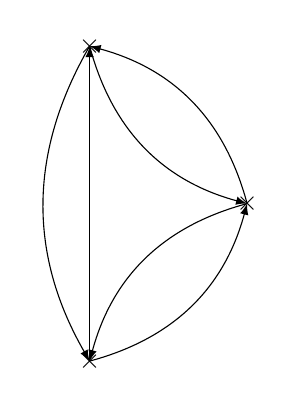
\begin{tikzpicture}
	\draw (0,4) node{$\times$} ;
	\draw [>=latex,->] (0,4) to[bend right] (2,2) ;
	\draw [>=latex,->] (2,2) to[bend right] (0,4) ;
	\draw (2,2) node{$\times$} ;
	\draw [>=latex,->] (0,0) to[bend right] (2,2) ;
	\draw [>=latex,->] (2,2) to[bend right] (0,0) ;
	\draw (0,0) node{$\times$} ;
	\draw [>=latex,->] (0,0) to (0,4) ;
	\draw [>=latex,->] (0,4) to[bend right] (0,0) ;
\end{tikzpicture}
\end{minipage}\hspace{0.1\linewidth}
\begin{minipage}{0.4\linewidth}
	Ici, on revient au même point en 2 ou 3 coups. On peut faire ça avec n'importe quel point, comme on l'a vu avec le théorème précédent. 
	$d=PGCD(2,3)=1$
\end{minipage}}

\subsection{Caractérisation}
\Theo{}{$\forall i\in C$, $N_{ii}=\{kd,\ k\in\mathbb{N}\textbackslash A_i\}$, $A_i$ fini.}

\begin{dem}
Quitte à diviser tous les éléments de $N_{ii}$ par $d$, on peut supposer que $PGCD(N_{ii})=1$ (pour simplifier).\\
$N_{ii}$ est un semi-groupe pour + :
	\[a,b\in N_{ii}\Rightarrow a+b\in N_{ii}\]

\bigskip
$N_{ii}\subset \mathbb{N}^*$\\
Donc $N_{ii}=\mathbb{N}\textbackslash A_i$, $A_i$ ensemble fini, ie $\exists k_i$ tel que $\forall n\geq k_i,\ n\in N_{ii}$.  (rien compris)

$N_{ii}\subset \mathbb{Z}$ et $PGCD (N_{ii})=1$, ce qui signifie que le module sur $\mathbb{Z}$ engendré par $N_{ii}$ est celui engendré par 1 qui est $\mathbb{Z}$. \\
(Après quelques recherches, il ne s'agirait pas d'un module mais plutôt d'un idéal)o

\[(N_{ii})=\left\{\sum_{k=1}^r \alpha_kn_k,\ \alpha_k\in\mathbb{Z}, n_k\in N_{ii}\right\}\]
$1\in (N_{ii})$\\
$\Rightarrow$ Identité de Bézout, i.e. $\exists n_1,...,n_r\in N_{ii}$, $a_1,...,a_r\in \mathbb{Z}$ tels que $a_1n_1+...+a_rn_r=1$.\\
On peut sopposer que $a_1,...,a_p>0$ et $a_{p+1},...,a_r\leq 0$.
	\[a_1n_1+...+a_pn_p=n\in N_{ii}\]
	\[m=-(a_{p+1}n_{p+1}+...+a_rn_r)\in N_{ii}\cup \{0\}\]

	$N_{ii}$ étant un semi-groupe pour + :
	\[\exists n\in N_{ii}, m\in N_{ii}\cup\{0\};\ n-m=1\]

	Si $m\neq 0$ :\\
Soit $k_i=m^2$. Si $k\geq m^2$
	\[k=m\alpha+\beta,\ \alpha\geq m,\ 0\leq \beta<m\]
\begin{eqnarray*}
	k&=&m\alpha+\beta(n-m)\\
	&=&\beta n+\underbrace{(\alpha-\beta)}_{>0}m
\end{eqnarray*}
Si $\beta=0$, $k=\alpha m\in N_{ii}$\\
Si $\beta>0$, $\beta n\in N_{ii}$ et $(\alpha-\beta)n\in N_{ii}$, donc $k\in N_{ii}$ ie 
	\[N_{ii}=\{\mathbb{N}\textbackslash \{0,...,m^2\}\}\]
\end{dem}

\Theo{}{$\forall i,j\in C$, $\exists r_{i,j}$, $0\leq r_{i,j}<d$ et \[N_{ij}=\{kd+r_{ij},\ k\in\mathbb{N}\textbackslash A_{ij}\] avec $A_{ij}$ un ensemble fini dépendant de $i$ et $j$.}

\begin{dem}
Montrons d'abord que deux éléments $a,b\in N_{ij}$ ont même reste dans la division par $d$.\\
Soient $a,b\in N_{ij}$, $c\in N_{ji}$.\\
$a+c$ et $b+c\in N_{ii}$ donc $a+c\equiv 0[d_i]$ et $c+b\equiv 0[d_i]$, donc $a+c-(b+c)=a-b\equiv 0[d_i]$. Donc $a$ et $b$ ont même reste dans la division par $d$.

\bigskip
Notons $r_{ij}$ ce reste commun à tous les éléments de $N_{ij}$. Tout élément $a$ de $N_{ij}$ s'écrit $a=kd+r_{ij}$.\\
Soit $k_i$ tel que $\forall l\geq k_i$, $ld\in N_{jj}$\\
Soit $a_0=k_0d+r_{ij}$, alors $\forall k\geq k_i$, $a_0+ld\in N_{ij}$\\
\[\forall l\geq k_i, (k_0+l)d+r_{ij}\in N_{ij}\]
\end{dem}

\subsection{Relation d'équivalence dans la classe $C$ et sous-classes périodiques}
\Def{}{Si $i,j\in C$, on dit que $i \sim j$ si et seulement s'il existe un chemin de longueur multiple de la période $d$ joignant $i$ à $j$\\
Cela se traduit par $i \sim j \Leftrightarrow r_{ij}=0$}

Cette relation est évidemment (hum) réflexive et transitive.\\
Pour la symétrie : si $r_{ij}=0$, soient $a\in N_{ji}$ et $b\in N_{ij}$. $a+b\in N_{jj}$ donc $a+b\equiv 0[d]$. \\
Or $b\equiv 0[d]$ car $r_{ij}=0$ donc $a\equiv 0[d]$ : $r_{ji}=0$.\\
Donc $C$ se partitionne en classes d'équivalences pour $\sim$. On les appelle les sous-classes cycliques.

\Theo{}{Si $d$ est la période de $C$ alors $C$ possède exactement $d$ sous-classes cycliques.\\
Celles-ci sont atteintes successivement toujours dans le même ordre tant que l'état du processus reste dans C.}

\section{Chaînes régulières}
\Def{}{On dit que la chaîne de Markov est régulière si et seulement si : 
\begin{enumerate}
	\item Elle ne possède qu'une seule classe
	\item Elle est apériodique (d=1)
\end{enumerate}}

\Theo{}{Les trois points suivants sont équivalents.
\begin{enumerate}
	\item La classe est régulière
	\item $\exists n_0,\ \forall n\geq n_0,\ \forall i,j\in E,\ \mathbb{P}(X_n=j|X_0=i)>0$
	\item $\exists n_0,\ \forall i,j\in E, \mathbb{P}(X_{n_0}=j|X_0=i)>0$
\end{enumerate}}

\begin{dem}
Il est clair que $2\Rightarrow 3$.\\
$3\Rightarrow 1$ car $\forall i,j\in N_{ij}=\mathbb{N}\textbackslash$ ens. fini. Donc $i\rightsquigarrow j$ et $r_{ij}=0$\\
$1\Rightarrow 2$ :
	\[\forall i,j \in N_{ij}\supset \{n>0,\ n\geq n_i\}\]
	($r_{ij}=0$ et $N_{ij}\neq \emptyset$)\\
	Soit $n_0=\max_{i\in E} (n_i)<+\infty$ (car E fini).\\
	$\forall i,j\in E, \exists n_0;\ \forall n\geq n_0, n\in N_{ij}$, ie $\mathbb{P}(X_n=i|X_0=i)>0$.
\end{dem}

\Lem{}{Soit $A=(a^i_j)_{i,j}$ une matrice "stochastique".\\
Soit $a^*=\min_{i,j} a^i_j>0$\\
Soit $X_0=(x_0^i)_i$ un vecteur colonne.\\
On pose $X_n=AX_{n-1}=A^nX_0$. Soit $M_n=\max_i x_n^i$ et $m_n=\min_i x_n^i$. \\
On a $m_n$ croissante, $M_n$ décroissante et $(M_n-m_n)\leq (1-2a^*)(M_0-m_0)$.}

\begin{dem}
\[x_{n+1}^i=\sum_j a_j^i x_n^j \geq \underbrace{\sum_j a_j^i}_{=1} m_n = m_n\]
Donc $m_{n+1}\geq m_n$, donc $m_n$ est croissante.\\
De même, $M_n$ est décroissante.

\bigskip
A présent, soit $j_0$ tel que $x_n^{j_0}=m_n$.
\begin{eqnarray*}
	x_n{n+1}^i &=& a_{j_0}^i m_n + \sum_{j\neq j_0} a_j^i x_n^j \\
		&\leq& a_{j_0}^i m_n + \underbrace{\left( \sum_{j\neq j_0} a_j^i\right)}_{=1-a^i_{j_0}} M_n \\
		&\leq& M_n-a^i_{j_0}(M_n-m_n)
\end{eqnarray*}

Donc \begin{equation}\tag{1} M_{n+1}\leq M_n-a^*(M_n-m_n)\end{equation}
En appliquant le résultat à $-X_n$ et à $-X_{n+1}$ :
\[-m_{n+1}\leq -m_n -a^*(-m_n-(-M_n))\]
\begin{equation} \tag{2} -m_{n+1}\leq -m_n -a^*(M_n-m_n) \end{equation}

\begin{eqnarray*} 
(1)+(2) : M_{n+1}-m_{n+1}&\leq& M_n-m_n-2a^*(M_n-m_n) \\
	M_{n+1}-m_{n+1}&\leq& (1-2a^*) (M_n-m_n)
\end{eqnarray*}
Par récurrence, on obtient le résultat.
\end{dem}

\Theo{fondamental}{On considère une chaîne de Markov régulière et E fini.\\
Dans ce cas, il existe une et une seule loi de probabilité invariante sur $E$. Notons la $\mu$. Celle-ci vérifie :
\begin{enumerate}
	\item $\forall i\in E$, $\mu_i>0$
	\item $\forall \mathcal{L}(X_0), \mathcal{L}(X_n)\to \mu$ exponentiellement vite 
	\item $\mu$ est l'unique solution de l'équation :
	\[\left\{\begin{array}{c c c}
		\nu \Pi &=& \nu\\
		\sum_{i\in E} \nu_i &=& 1
	\end{array}\right.\]
\end{enumerate}}

\begin{dem}
Considérons la colonne $j$ de $\Pi^n$ : $C_j^n$.\\
Que devient-elle lorsque $n\to +\infty$ ?
\[\begin{array}{c c c c c}
C_j^0=\begin{pmatrix} 0\\ \vdots \\ 1 \\ 0 \\ \vdots \end{pmatrix} \text{jième ligne} & \hspace{4em} C_j^n &=& \Pi^n C_j^0 \\
& &=&\Pi C_j^{n-1}
\end{array}\]

Soit $M_j^n=\max_i (C_j^n)_i$ et $m_j^n = \min_i (C_j^n)_i$. \\
On a $M_j^n$ décroissante, $m_j^n$ croissante et $m_j^n\leq M_j^n$. \\
Comme $M_j^n\geq m_j^0$, $M_j^n$ converge. De même, $m_j^n$ converge également.

\bigskip
Montrons que $M_j^n-m_j^n\to l_j=0$.\\
Soit $n_0$ tel que $A=\Pi^{n_0}$ soit à termes positifs (cela signifie que la chaîne est régulière, d'après le premier théorème de cette section).\\
Soit $p^*=\min_{i,j} (p_j^i(n_0))>0$. On a :
\[M_j^{kn_0}-m_j^{kn_0}\leq (1-2p^*)^k\underbrace{(M_j^0-m_j^0)}_{=1}\xrightarrow[k\to +\infty]{} 0\]
Donc la sous-suite $(M_j^{kn_0}-m_j^{kn_0})_k$ de $(M_j^{n}-m_j^{n})_n)$ converge vers 0. Or, la suite est convergente vers $l_j$, donc $l_j=0$.\\
Donc $M_j^n$ et $m_j^n$ ont même limitE. Notons la $\mu_j$.
\[C_j^n=(p_j^i(n))_i \to \begin{pmatrix} \mu_j \\ \vdots \\ \mu_j \end{pmatrix}\]
\[\Pi^n \to \begin{pmatrix} \mu_1 & \cdots & \mu_n \\ \vdots & \ddots & \vdots \\ \mu_1 & \cdots & \mu_n \end{pmatrix}\]

\[\mu_j\geq m_j^{n_0}\geq p^* >0\]
\[\forall j,\ \mu_j>0\]
\[m_j^n\leq \mu_j \leq M^n_j\]
\begin{eqnarray*}
	|\mu_j-p^i_j(n)|&\leq& M_j^n-m_j^n \\
			&\leq& M_j^{kn_0+r}-m_j^{kn_0+r} \\
			&\leq& (1-2p^*)^k (M_j^r-m_j^r)\\
			&\leq& \left((1-2p^*)^{\frac{1}{n_0}} \right)^{kn_0}(1-2p^*)^{\frac{r}{n}} \underbrace{\max_{r<n_0, j} \frac{M_j^r-m_j^r}{(1-2p^*)^{\frac{r}{n_0}}}}_{=a}\\
			&\leq& a\left[ (1-2p^*)^{\frac{1}{n_0}}\right]^n
\end{eqnarray*}
Si $b=(1-2p^*)^{\frac{1}{n_0}}$, $0\leq b<1$
\[\forall j,\ |\mu_j-p_j^i(n)|\leq ab^n\]
On a donc une convergence exponentielle de $\mathbb{P}(X_n=j|X_0=i)$ vers $\mu_j$

\bigskip
Soit $\nu^0$ loi de $X_0$.\\
\begin{eqnarray*}
\mathbb{P}(X_n=j)&=&\sum_i \mathbb{P}(X_n=j|X_0=i)\mathbb{P}(X_0=i) \\
		&=& \sum_i \nu_i^0 p_j^i(n)
\end{eqnarray*}
Comme $\sum_i \nu_i^0=1$ :
\begin{eqnarray*}
|\mathbb{P}(X_n=j)-\mu_j|&=&\left| \sum_i \nu_i^0 (p^i_j(n)-\mu_j)\right|\\
			&\leq&\sum_i \nu_i^0 |p_j^i(n)-\mu_j| \\
			&\leq&\sum_i \nu_i^0 ab^n\\
			&\leq& ab^n
\end{eqnarray*}
$\forall \mathcal{L}(X_0)$, $\mathcal{L}(X_n)\to\mu$ exponentiellement vite, ie \[|\mathbb{P}(X_n=j)-\mu_j|\leq ab^n\]
$\mu$ est une loi de probabilité :
\[1=\sum_{j\in E} \mathbb{P}(X_n=j|X_0=i) \to \sum_{j\in E} \mu_j = 1\]
Donc $\forall j,\ \mu_j\geq p^*>0$ et $\sum_i \mu_j=1$.

\bigskip
Soit $\nu$ un vecteur ligne.
\[\nu\Pi^n \to \nu \begin{pmatrix} \mu_1 & \cdots & \mu_n \\ \vdots & \ddots & \vdots \\ \mu_1 & \cdots & \mu_n \end{pmatrix} = \left( \sum_i \mu_i \nu_1\ \cdots\ \sum_i \nu_i \mu_n \right) = \left( \sum_i \nu_i \right) \mu\]

\[\forall \nu,\ \nu\Pi^n \to \left( \sum_i \nu_i \right) \mu\]
Donc $\mu\Pi^n\to \mu$, donc $\left( \mu\Pi^n\right) \Pi \to \mu\Pi$, donc \[\mu\Pi=\mu\]

$\mu$ est donc une loi e probabilité invariante. C'est la seule loi de probabilité invariante :\\
Si $\nu$ est une loi de probabilité invariante, alors $\nu\Pi=\nu$. Donc $\forall n\ \nu\Pi^n=\nu$. Or, $\nu\Pi^n\to \mu$ donc $\nu=\mu$

\bigskip
$\mu$ vérifie $\mu\Pi=\mu$, $\sum_i \mu_i =1$. Soit $\nu$ solution de $\nu\Pi=\nu,\ \sum_i \nu_i=1$. Aors :
\[\nu \Pi^n = \nu \to \left(\sum_i \nu_i\right) \mu = \mu\]
Donc $\mu=\nu$.
\end{dem}

\subsection{Conséquences}
\begin{enumerate}
\item Supposons que sur E, il n'y ait qu'une seule classe finale et que celle-ci soit apérioique (d=1). Que devient $\mathcal{L}(X_n)$ lorsque $n\to +\infty$ ?\\
\begin{center}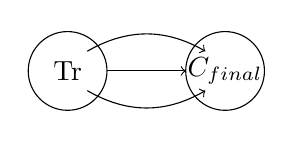
\begin{tikzpicture}
	\draw (-0.5,0) circle(0.5);
	\draw (-0.5,0) node{Tr};
	\draw (1.5,0) circle(0.5);
	\draw (1.5,0) node{$C_{\text{final}}$};
	\draw [->] (0,0)--(1,0);
	\draw [->] (-0.25,-0.25) to[bend right] (1.25,-0.25);
	\draw [->] (-0.25,0.25) to[bend left] (1.25,0.25);
\end{tikzpicture}\end{center}
$\mathcal{L}(X_n)\to \mu_C$, où $\mu_C(j)=0$ $\forall j\in Tr$.\\
$\mu_{C_{|C}}$ = loi de probabilité invariante de la chaîne quand elle début dans C.\\
Sur C, $X_n$ est une chaîne régulière.\\
$\mu=\mu_{C_{|C}}$ vérifie $\mu A=\mu$, $\sum_i \mu_i=1$, dont elle est l'unique solution.
\end{enumerate}

\Theo{ergodique (admis)}{Supposons que la chaîne n'ait qu'une seule classe finale $C$ et que celle-ci est apériodique.\\
Soit $\mu$ la mesure invariante sur $C$ décrite précédemment. Alors :
\[\forall f:E\to \mathbb{R},\ \frac{1}{n} \sum_{k=0}^{n-1} f(X_k) \xrightarrow[\forall \mathcal{L}(X_0)]{p.s.} \int_C f d\mu = \sum_{j\in C} f(j)\mu(j)\]}

\subsection{Etude d'une classe finale périodique}
Soit $d$ la période d'une classe $C$, finale. Elle possède $d$ sous-classes cycliques, parcourues successivement, toujours dans le même ordre. Numérotons les de A à $d$ de façon qu'on les parcourt ainsi :\\
\begin{center}\begin{tikzpicture}
	\draw [->] (0,3)--(1,3);
	\draw (1,5) rectangle (5,1);
	\draw (2,3) node{$C_d$};
	\draw (3,4) node{$C_1$};
	\draw [->] (2.1,3.1) to[bend left] (2.9,3.9);
	\draw (4,3) node{$C_2$};
	\draw [->] (3.1,3.9) to[bend left] (3.9,3.1);
	\draw (3,2) node{$C_k$};
	\draw [->] (3.9,2.9) to[bend left] (3.1,2.1);
	\draw [->] (2.9,2.1) to[bend left] (2.1,2.9);
	\draw (5,1) node[right]{$C$};
\end{tikzpicture}\end{center}

$\Pi$ s'écrit alors :
\[\Pi=\begin{pmatrix} 0 & A_1 & 0 & \cdots & 0 \\
		      0 & 0 & A_2 & \cdots & 0 \\
		      \vdots & \ddots & \ddots & \ddots & \vdots \\
		      0 & 0 & 0 & \cdots & A_{d-1} \\
		      A_d & 0 & 0 & \cdots & 0 \end{pmatrix}\]
\[\Pi^d=\begin{pmatrix} B_1 & 0 & \cdots & 0 \\
			0 & B_2 & \cdots & 0 \\
			\vdots & \vdots & \ddots & \vdots \\
			0 & 0 & \cdots & B_d\end{pmatrix}\]

Avec : \begin{eqnarray*}
	B_1 &=& A_1 \cdots A_d \\
	B_2 &=& A_2 \cdots A_d A_1 \\
	\vdots \\
	B_k &=& A_k \cdots A_d A_1 \cdots A_{k-1} \\
	\vdots \\
	B_d &=& A_d A_1 \cdots A_{d-1}
\end{eqnarray*}

Si on considère $C_k$, $B_k$ est la matrice de transition sur $C_k$. C'est une chaîne de Markov régulière.\\
Elle admet une unique loi de probabilité invariante $\mu_k$ concentrée sur $C_k$. 
	\[\left\{ \begin{array}{c c c} \mu_k B_k &=& \mu_k \\ \sum_{i\in C_k} \mu_k(i) &=& 1 \end{array} \right.\]

\Theo{}{Il existe une unique mesure de probabilité invariante sur C. Notons la $\mu$. On a :
	\[\mu=\frac{1}{d} \left(\mu_1,...,\mu_d \right)\]
$\mu_k$ : vecteur ligne indéxée par $C_k$.}

\begin{dem}
Montrons que $\mu=\frac{1}{d}(\mu_1,...,\mu_d)$ est une mesure de probabilité invariante.
	\[\mu \Pi = \frac{1}{d} (\mu_dA_d , \mu_1A_1, ... , \mu_{d-1}A_{d-1}\]
$\mu_k A_k$ est une mesure de probabilité sur $C_{k+1}$. 
\begin{eqnarray*}
\mu_kA_kB_{k+1}&=&\mu_kA_kA_{k+1}...A_dA_1...A_k \\
		&=& \mu_k B_k A_k\\
		&=& \mu_k A_k
\end{eqnarray*}
Donc $\mu_k A_k=\mu_{k+1}$ par unicité de la loi de probabilité invariante concentrée sur $C_{k+1}$. Donc $\mu\Pi=\mu$.\\
$\mu$ est donc une loi de probabilité invariante.

\bigskip
Prouvons à présent son unicité.\\
Soit $\nu$ une mesure de probabilité invariante.
	\[\nu=(\nu_1,...,\nu_k,...,\nu_d), \nu_k=(\nu_i)_{i\in C_k}\]
	\[\sum_{i\in C_k} \nu_k(i) = \nu(C_k)\]

On a $\nu\Pi=\nu$ donc $\nu\Pi^d=\nu$. donc $\forall k, \nu_kB_k=\nu_k$. Donc :
	\[\frac{\nu_k}{\nu(C_k)} = \mu_k \text{ (par unicité)}\]
Donc $\nu_k=\nu(C_k)\mu_k$.\\

\bigskip
Il reste à montrer que $\forall k$, $\nu(C_k)=\frac{1}{d}$, ie 
	\[\forall k,l, \nu(C_k)=\nu(C_l)\]
car
	\[\sum_{k=1}^d \nu(C_k)=1\]
On a $\nu\Pi=\nu$, donc ::
	\begin{eqnarray*}
		\nu_dA_d&=&\nu_1 \\
		\nu_1A_1&=&\nu_2 \\
		\vdots \\
		\nu_kA_k &=& \nu_{k+1}
	\end{eqnarray*}
\[(\nu_kA_k)_j=\sum_{i\in C_k} \nu_k(i) a_j^i\]
\[\sum_{j\in C_{k+1}} (\nu_k A_k)_j = \sum_{i\in C_k} \nu_k(i) \sum_{j\in C_{k+1}} a^i_j = \sum_{i\in C_k} \nu_k(i) = \nu(C_k)\]
Or, $\nu_kA_k=\nu_{k+1}$ et $\sum_{i\in C_{k+1}} \nu_{k+1}(i)=\nu(C_{k+1})$, donc 
	\[\forall k, \nu(C_k)=\nu(C_{k+1})\]
Ils sont donc tous égaux à $\frac{1}{d}$.
\end{dem}

\Rem{}{\begin{itemize}
	\item Pour cette loi invariante $\mu$, chaque classe $C_k$ a même probabilité $\mu(C_k)=\frac{1}{d}$
	\item Pour trouver $\mu$, 2 méthodes :
	\begin{itemize}
		\item $\mu$ solution de $\mu\Pi=\mu$ et $\sum_{i\in C} \mu_i=1$
		\item On calcule $\Pi^d=diag(B_1,...,B_d)$ et on résout $\mu_kB_k=\mu_k,\ \sum_{i\in C_k} \mu_k(i)=1$. Puis $\mu=\frac{1}{d} (\mu_1,...,\mu_d)$.
	\end{itemize}
	\item Dans la démonstration, au lieu de supposer $\nu$ probabilité invariante, on aurait pu supposer 
		\[\left\{ \begin{array}{c} \nu \text{ solution de } \nu\Pi=\nu \\ \sum \nu_i = 1 \end{array}\right.\]
		Le reste est inchangé.
\end{itemize}}

\Theo{ergodique}{Supposons que la chaîne ne possède qu'une seule classe finale $C$. Soit $\mu_C$ la mesure invariante associée à cette classe. $\forall f:E\to\mathbb{R}$ (E fini) :
\[\frac{1}{n} \sum_{k=1}^n f(X_k) \xrightarrow[\forall \mathcal{L}(X_0)]{p.s.} \int_C f d\mu_C = \sum_{i\in C} f(i)\mu_C(i)\]}

\part{Programmation lin\'eaire, algotihme du simplexe}
\section{Introduction}
Un problème d'optimisation linéaire est un problème d'optimisation dans lequel le coût et les contraintes sont linéaires (ou plutôt affines).\\
Il s'agit de trouver les solutions $x\in\mathbb{R}^n$ du problème :
\begin{equation}\tag{$P_L$} \label{PL}
	\left\{ \begin{array}{c c c c} \inf_{x\in\mathbb{R}^n} & \multicolumn{3}{c}{\langle c,x\rangle} \\
						\text{s. c.}     & Ax &=& b \\
								& x &\geq& 0
	\end{array} \right.
\end{equation}

où $A$ est une matrice de raille $m\times n$, $b\in\mathbb{R}^m$, $c\in\mathbb{R}^n$.\\
$x\geq 0$ signifie que toutes les composantes de $x$ sont positives.\\
Ce problème est dit sous forme standard.

\bigskip
\underline{Remarque :} On a l'impression que \ref{PL} est un cas particulier du problème (sous forme canonique) : 
\begin{equation} \label{PC}
	\left\{ \begin{array}{c c c c} \inf_{x\in\mathbb{R}^n} & \multicolumn{3}{c}{\langle c,x\rangle} \\
						\text{s. c.}     & A'x &=& b' \\
								& Ax &\geq& b
	\end{array} \right.
\end{equation}

Mais un problème sous forme canonique peut toujours se ramener à un problème sous forme standard. En effet, la contrainte $A'x=b'$ est équivalent à $A'x\geq b'$ et $-A'x\geq -b'$. Donc \ref{PC} est équivalent à :
\begin{equation} \label{PC2} \inf_{x\in\mathbb{R}^n,\ Ax\geq b} \langle c,x\rangle\end{equation}

On introduit des variables d'écart $\lambda\in\mathbb{R}^n_+$ tel que $Ax=b+\lambda$. Donc \ref{PC2} se ramène à :
\[	\left\{ \begin{array}{c c c c} \inf_{x\in\mathbb{R}^n,\ \lambda\in\mathbb{R}^n_+} & \multicolumn{3}{c}{\langle c,x\rangle} \\
						\text{s. c.}     & Ax-\lambda &=& b \\
								& b &>& 0
	\end{array} \right.\]

On décompose $x$ sous la forme :
	\[x=x^+-x^-\]
où $x^+=\max (0,x) \geq 0$ et $x^-=-\min (0,x)\geq 0$ \\
\ref{PC2} revient donc à résoudre :
\[	\left\{ \begin{array}{c c c c} \inf_{x^+\in\mathbb{R}^n, x^-\in\mathbb{R}^n, \lambda\in\mathbb{R}^n}& \multicolumn{3}{c}{\langle c,x\rangle} \\
						\text{s. c.}     & Ax-\lambda &=& b \\
								& b &>& 0
	\end{array} \right.\]
qui est bien sous forme standard (mais avec plus de variables).

\bigskip
\underline{Remarque :} On peut supposer sans perte de généralité que toutes les lignes de $A$ sont linéairement indépendantes.\\
Si ce n'est pas le cas, soit certaines constraintes sont redondantes, soit les contraintes sont incompatibles, ie $rg(A)=m\leq n$

\Def{}{L'ensemble \[X_{ad}=\{x\in\mathbb{R}^n,\ Ax=b,\ x\geq 0\}\]
est appelé l'ensemble des solutions réalisables (ou admissibles).\\
On appelle sommet (ou point extremal) de $X_{ad}$ un point $x\in X_{ad}$ tel qu'il n'existe pas $\alpha\in]0,1[$ et $y,z\in X_{ad}$, $y\neq z$ tel que $x=\alpha y+(1-\alpha)z$.}

\section{Solutions de base d'un problème sous forme standard}
On note $A_1=\begin{pmatrix} a_{1,1} \\ \vdots \\ a_{m,1} \end{pmatrix}$, ..., $A_n=\begin{pmatrix} a_{1,n} \\ \vdots \\ a_{m,n} \end{pmatrix}$. \\
Comme $rg(A)=m$, on peut toujours trouver $m$ colonnes de $A$ linéairement indépendantes.\\
On note
	\[\Gamma=\{\gamma:\{1,...,m\}\to \{1,...,n\}, \text{ strictement croissante} \}\]
On définit :
	\[A_{\gamma}=(A_{\gamma(1)} \cdots A_{\gamma(m)})\]
et :
	\[\mathcal{B}=\{\gamma\in\Gamma,\ rg(A_{\gamma})=m\}\]

Pour $\gamma\in\Gamma$, on définit $\hat{\gamma}$ comme l'unique application strictement croissante de $\{1,...,n-m\}$ dans $\{1,...,n\}$ tel que :
	\[\gamma(\{1,...,m\})\cup\gamma(\{1,...,n-m\})=\{1,...,n\}\]

\Def{}{Pour $\gamma\in\mathcal{B}$, la matrice $A_{\gamma}$ est appelée base associée à $\gamma$.\\
Les composantes $(x_{\gamma(1)},...,x_{\gamma(m)})$ sont appelées les composantes de base, et les composantes $(x_{\hat{\gamma}(1)},...,x_{\hat{\gamma}(n-m)})$ sont appelées les composantes hors base.}

Pour $\gamma\in\mathcal{B}$, on note
	\[x_{\mathcal{B}}=(x_{\gamma(1)},...,x_{\gamma(m)})\]
	\[x_{N}=(x_{\hat{\gamma(1)}},...,x_{\hat{\gamma(m)}})\]
	\[B=A_{\gamma}\]
	\[N=A_{\hat{\gamma}}\]
\[Ax=Bx_{\mathcal{B}}+Nx_N\]

Comme $rg(B)=rg(A_{\gamma})=m$, B est inversible. Donc les contraintes $Ax=b$ peuvent se réécrire :
	\[Bx_{\mathcal{B}}=b-Nx_N\]
	\[\Rightarrow B^{-1}(b-Nx_N)\]

\Def{}{Soit $\gamma\in\mathcal{B}$, on appelle solution de base du système $Ax=b$ associé à la base $\gamma$ la solution $x^*$ définie par :
	\[\begin{array}{c c c}
	x_{\mathcal{B}}^*&=&B^{-1}b\\
	x_N^*&=&0
	\end{array}\]}


\Def{}{Une solution de base réalisable est une solution de base tel que $x_{\mathcal{B}}\geq0$ ($\rightarrow x^*\in X_{ad}$).\\
Dans ce cas, $\gamma$ est appelée base réalisable. On note $\mathcal{R}$ l'ensemble des bases réallisables.\\
Enfin on dit que $x^*$ est non dégénéré si $x_{\mathcal{B}}^*>0$ (ie $B^{-1}b>0$).}

\Lem{}{Les sommets de $X_{ad}$ sont exactement les solutions de base réalisable.}

\begin{dem}
Soit $x^*$ une solution de base réalisable associée à la base $\gamma\in\mathcal{R}$.\\
Par l'absurde, on va supposer que $x^*$ n'est pas un sommet de $X_{ad}$/ 
	\[\forall \theta\in]0,1[, \exists y,z\in X_{ad}, y\neq z; x^*=\theta y+(1-\theta)z\]
$\forall i\in\{0,...,n-m\}$, on a :
	\[x_{\hat{\gamma}(i)}=0=\underbrace{\theta}_{>0} \underbrace{y_{\hat{\gamma}(i)}}_{\geq 0} + \underbrace{(1-\theta)}_{>0}\underbrace{z_{\hat{\gamma}(i)}}_{\geq 0}\]

	\[\Rightarrow y_{\hat{\gamma}(i)}=z_{\hat{\gamma}(i)}=0\]
	\[\Rightarrow y_N=z_N=0\]

Or, $y_B=B^{-1}(b-Ny_N)=B^{-1}b=z_B=x^*_B$. Donc $y=z=x^*$, ce qui est absurde.\\
Donc $x^*$ est un sommet de $X_{ad}$.

\bigskip
Réciproquement, on suppose que $x^*$ est un sommet de $X_{ad}$. On note $k$ le nombre de composantes non nulles de $x^*$. 
\[\exists \gamma_1 : \{1,...,k\}\to\{1,...,n\} \text{ strictement croissante telle que } x^*_{\gamma_1(i)}>0,\ \forall i=1,...,k\]
On veut montrer que les vecteurs $A_{\gamma_1(1)},...,A_{\gamma_1(k)}$ sont libres. Si c'est le cas, on pourra compléter cette famille de vecteurs afin d'obtenir une base.\\
($\Rightarrow$ On définit $\gamma\in\Gamma$ telle que :\begin{itemize}
\item $\gamma_1(\{1,...,k\}\subset\gamma(\{1,...,m\})$
\item $\gamma\in\mathcal{B}$
\end{itemize})

Par l'absurde, on suppose que $A_{\gamma_1(1)},...,A_{\gamma_1(k)}$ sont liés. Alors $\exists y\in\mathbb{R}^n$, $y\neq 0$, 
\[\sum_{i=1}^k y_{\gamma_1(i)}A_{\gamma_1(i)}=0\]
et \[y_{\hat{\gamma}_1(i)}=0\]
$\forall \varepsilon>0$, on a \[A(x+\varepsilon y)=Ax+\varepsilon \underbrace{Ay}_{=0}=b\]
\[A(x-\varepsilon y)=Ax-\varepsilon Ay = b\]
On a $x^*_{\gamma_1(i)}\pm \varepsilon y_{\gamma_1(i)}>0$, $\forall i=1,...,k$ pour $\varepsilon$ assez petit.\\
De plus, $x^*_{\hat{\gamma}_1(i)}\pm \varepsilon y_{\hat{\gamma}_1(i)}=x^*_{\hat{\gamma}_1(i)}=0$
	\[\Rightarrow x^*+\varepsilon y\in X_{ad},\ \forall0\leq \varepsilon \leq \varepsilon_0\]
Or, $x^*=\frac{1}{2}(x^*+\varepsilon y) + \frac{1}{2}(x^*-\varepsilon y)$. Donc $x^*$ n'est pas un sommet de $X_{ad}$. Contradiction.
\end{dem}

\Lem{}{S'il existe une solution optimale de $(P_L)$ alors il existe une solution optimale de base réalisable.}

\begin{dem}
Soit $x\in X_{ad}$ une solution optimale. On note $k$ le nombre de composantes non nulles de $x$. Soit $\gamma_1:\{1,...,k\}\to \{1,...,n\}$ strictement croissante telle que $x_{\gamma_1(i)}>0$ $\forall i=1,...,k$.\\
Si la famille $A_{\gamma_1(1)},...,A_{\gamma_1(k)}$ est libre alors $x$ est une solution optimale de base réalisable.\\
Si la famille $A_{\gamma_1(1)},...,A_{\gamma_1(k)}$ est liée, alors $\exists y\in\mathbb{R}^n$ tel que :
	\[\sum_{i=1}^k y_{\gamma_1(i)} A_{\gamma_1(i)}=0\]
	\[y_{\hat{\gamma}_1(i)}=0\ \forall i 1\leq i\leq n-k\]
$x+\varepsilon y\in X_{ad}$ pour $\varepsilon$ assez petit (cf démo précédente). \\
Comme $c$ est un point de minimum, on a :
	\[\langle c,x\rangle \leq \langle c, x\pm \varepsilon y\rangle\]
	\[\Rightarrow \pm\langle c, y\rangle \geq 0\]
	\[\langle c,y\rangle=0\]
On pose $\varepsilon_1=\sup\{\varepsilon>0;\ x\pm\varepsilon y\in X_{ad}\}$. 
	\[\exists i\in \{1,...,k\} \text{ tel que } (x+\varepsilon y)_{\gamma_1(i)}=0 \text{ ou } (x-\varepsilon y)_{\gamma_1(i)}=0\]
On pose $z=x+\varepsilon y$ ou $z=x-\varepsilon$. tel que $z_{\gamma_1(i)}=0$. z est donc une solution otpimale 
\[(\langle c,z\rangle=\langle c,x\pm\varepsilon y\rangle = \langle c,x\rangle)\]
qui a au plus $k-1$ composantes non nulles.\\
On peut refaire la preuve en remplaçant $x$ par $z$ (et en diminuant $k$) jusqu'à obtenir une famille libre.
\end{dem}

\part{Processus d'entrée-sortie}
On considère un système dans lequel des "objets" rentrent, y restent un certain temps aléatoire et en repartent.\\
$X_t$ : le nombre d'objets présents à $t$ dans le système.

\section{Cadre général}
\subsection{Hypothèses et paramètres, générateur infinitésimal}
On peut distinguer deux cas :
\begin{itemize}
	\item Capacité limité : $X_t\leq N$ : espace d'états fini
	\item Capacité illimité : $X_t\in\mathbb{N}$
\end{itemize}

\bigskip
$S$ : instant d'arrivée du premier objet après $t=0$\\
$T$ : instant de départ du premier objet après $t=0$

\bigskip
Si $0<k<N$ (ou $k>0$ si illimité) : $S$ et $T$ sont indépendantes sachant que $X_0=k$.
	\[\mathcal{L}(S|X_0=k)=\mathcal{E}(\alpha_k) \hspace{3em} \mathcal{L}(T|X_0=k)=\mathcal{E}(\beta_k)\]
Les $\alpha_k$ et les $\beta_k$ sont les paramètres du modèle.
	\[\mathbb{P}(S=T|X_0=k)=0\]
$U=S\cap T$ : instant de première transition.
	\[\mathcal{L}(Y|X_0=k)=\mathcal{E}(\alpha_k+\beta_k)\]
donc $a_k=-a_k^k=\alpha_k+\beta_k$.
	\[\hat{p}^k_{k+1}=\mathbb{P}(S<T|X_0=k)=\frac{\alpha_k}{\alpha_k+\beta_k}=\frac{a^k_{k+1}}{a_k}\]
donc $a^k_{k+1}=\alpha_k$ et de même, $a^k_{k-1}=\beta_k$

\bigskip
Si $k=0$ : $S=U$
	\[\mathcal{L}(S|X_0=0)=\mathcal{E}(\alpha_0)\]
	\[a_0=\alpha_0\]
	\[\hat{p}_1^0=1\Rightarrow a_1^0=\alpha_0\]
Si $k=N$ (capacité limitée) : $T=U$
	\[\mathcal{L}(T|X_0=0)=\mathcal{E}(\beta_N)\]
	\[a_N=\beta_N\]
	\[\hat{p}_{N-1}^N=1\Rightarrow a_{N-1}^N=\beta_N\]

\[A=\begin{pmatrix}-\alpha_0 &      \alpha_0       &    0     & \cdots & \cdots & \cdots & 0 \\
		    \beta_1  & -(\alpha_1+\beta_1) & \alpha_1 &    0   & \cdots & \cdots & 0 \\
		     \vdots  &      \ddots         &  \ddots  & \ddots &        &        & \vdots \\
                    \vdots   &                     &  \ddots  & \ddots & \ddots &        & \vdots \\
		    \vdots   &                     &          & \ddots & \ddots & \ddots & \vdots \\
                       0     &       \cdots        &  \cdots  & \cdots &   0    &\beta_N & -\beta_N \end{pmatrix}\]

\subsection{Classification, recherche de lois de probabilité invariante}
On constate que $\forall k,l$, $k\rightsquigarrow l$. On a donc une seule classe.\\
On a une chaîne régulière (en temps continu). 
\begin{itemize}
	\item Si capacité limitée : chaîne régulière, espace d'état fini
	\item Si capacité illimitée, on a une chaîne régulière dans un espace d'état inifini dénombrable.
\end{itemize}

La loi de probabilité invariante existe et est unique dans le cas fini.
	\[\mu \text{ doit vérifier } \left\{ \begin{array}{c c c} \mu A&=&0 \\ \sum_i \mu_i &=& 1 \end{array} \right.\]

$\mu=(x_0....x_N)$
	\[-\alpha_0x_0+\beta_1x_1=0\]
	\[\alpha_0x_0-(\alpha_1+\beta_1)x_1+\beta_2x_2=0\]
	\[\alpha_1x_1-(\alpha_2+\beta_2)x_2+\beta_3x_3=0\]
	\[...\]

	\[x_1=\frac{\alpha_0}{\beta_1}x_0\]
	\[x_2=\frac{\alpha_0\alpha_1}{\beta_1\beta_2}x_0\]
	\[...\]
	\[x_k=\frac{\alpha_0...\alpha_{k-1}}{\beta_1...\beta_k}x_0\]

$E=\{0,...,N\}$ ou $E=\mathbb{N}$.\\
Soit $C=1+\sum_{k\in E} \frac{\alpha_0...\alpha_{k-1}}{\beta_1...\beta_k}$. On doit avoir $x_0 C=1$.\\

\begin{itemize}
	\item Si $E$ fini, alors $C<+\infty$ et $x_0=\frac{1}{C}$.
	\[x_k=\mu_k=\frac{1}{C}\frac{\alpha_0...\alpha_{k-1}}{\beta_1...\beta_k}\]
et $\mathcal{L}(X_0)$, $\mathcal{L}(X_t)\to \mu$ exponentiellement vite.

	\item Si $E=\mathbb{N}$, \begin{itemize}
		\item Si $C=+\infty$, il n'existe pas de loi de probabilité invariante. Par contre, il existe une unique mesure ($\sigma$-finie) invariante (à une constante multiplicative près) $\mu$ donnée par $\mu_k=\frac{\alpha_0,...,\alpha_{k-1}}{\beta_1....\beta_k}$. On a ici un phénomène d'explosion.
		\item Si $C<+\infty$,, alors il existe une et une seule loi de probabilité invariante $\mu$ donnée par $\mu_k=\frac{1}{C}\frac{\alpha_0...\alpha_{k-1}}{\beta_1...\beta_k}$. On montre qu'alors $\mathcal{L}(X_t)\to \mu$ et le théorème ergodique reste vrai dans ce cas.
	\end{itemize}
\end{itemize}

\section{Processus de Poisson}
On considère une suite de phénomènes survenant à des instants aléatoires $T_0=0<T_1<...<T_n<...$ avec $T_n\xrightarrow[n\to +\infty]{} +\infty$
\Def{Processus de comptage associé}{$N_t$ : le nombre de phénomène survenus dans l'intervalle de temps $]0,t]$ $(N_0=0)$\\
On suppose que $N_t$ ne croit que par sauts de 1 (ie 2 phénomènes ne peuvent être simultanés).}

Les lois de $N_t$ et de $T_k$ sont liées. \[\mathbb{P}=(N_t\leq k)=\mathbb{P}(T_k\geq t)\]

\subsection{Hypothèse des processus de Poisson}
On suppose que $N_t$ (processus de comptage) : \begin{enumerate}
	\item est à accroissements indépendants : $N_t-N_s\Inde (N_u,\ u\leq s)$ (ie le nombre d'évènements surevnus entre $s$ et $t$ est indépendant de ce qui s'est passé avant $s$)
	\item est à avancement stationnaire : $\mathcal{L}(N_t-N_s)$ ne dépend que de la durée $t-s$.
		\[\mathcal{L}(N_t-N_s)=\mathcal{L}(N_{t-s}-N_0)=\mathcal{L}(N_{t-s})\]
\end{enumerate}

\Theo{}{Sous les hypothèses précédentes, il existe $\lambda>0$ tel que :
	\[\forall t,\ \mathcal{L}(N_t)=\mathcal{P}(\lambda t) \text{ (Loi de Poisson de paramètre }\lambda t)\]
	\[\forall k\in\mathbb{N},\ \mathbb{P}(N_t=k)=\frac{(\lambda t)^k}{k!} e^{-\lambda t}\]
	\[\mathbb{E}(N_t)=\lambda t \text{ : nombre moyen d'évènements surevnus dans un intervalle de temps de longueur t}\]
}

\begin{dem}
Posons $p_k(t)=\mathbb{P}(N_t=k)$.
$\bullet$ Calcul de $p_0(t)$ :
	\[\mathbb{P}(N_{t+h}=0)=\mathbb{P}(N_{t+h}-N_t=0,N_t=0)\]
Par indépendance :
	\[\mathbb{P}(N_{t+h}=0)=\mathbb{P}(N_{t+h}-N_t=0)\mathbb{P}(N_t=0)\]
Donc $\forall s,t>0$ :
	\[\begin{array}{c} p_0(t+s)=p_0(t)p_0(s) \\ p_0(t) \text{ décroit} \end{array}\Leftrightarrow \exists \lambda>0; p_0(t)=e^{-\lambda t}\]

\bigskip
$\bullet$ Calcul de $p_k(t),\ k\geq 1$ :
On admettra que $\mathbb{P}(N_h\geq 2)=o(h)$\\
$p_k(t+h)=\mathbb{P}(N_{t+h}=k)$ (avec $h$ petit).
\begin{eqnarray*}
p_k(t+h)&=&\mathbb{P}(N_t=k,N_{t+h}-N_t=0)+\mathbb{P}(N_t=k-1,N_{t+h}-N_t=1)+\sum_{k\leq k-2} \mathbb{P}(N_t=j,N_{t+h}-N_t=k-j)\\
	&=&\mathbb{P}(N_t=k)\mathbb{P}(N_{t+h}-N_t=0)+\mathbb{P}(N_t=k-1)\mathbb{P}(N_{t+h}-N_t=1)+o(h)\\
	&=&p_0(h)p_k(t)+p_1(h)p_{k-1}(t)+o(h)
\end{eqnarray*}

Or, $p_0(h)+p_1(h)+\mathbb{P}(N_h\geq 2)=1$\\
$e^{-\lambda h}+p_A(h)+o(h)=1$\\
$1-\lambda h+o(h)+p_1(h)+o(h)=1$
\[\Rightarrow \left\{\begin{array}{c c c} p_1(h)&=&\lambda h+o(h) \\ p_0(h)&=&1-\lambda h+o(h) \end{array}\right.\]

\[p_k(t+h)=(1-\lambda h)p_k(t)+\lambda hp_{k-1}(t)+o(h)\]
\[\frac{1}{h}\left( p_k(t+h)-p_k(t)\right)=-\lambda p_k(t)+\lambda p_{k-1}(t)+o(1)\]
\[\begin{array}{c} p_k'(t)=\lambda(-p_k(t)+p_{k-1}(t),\ k\geq 1\\ p_0(t)=e^{-\lambda t} \end{array}\]

Variation de la constante : posons $p_k(t)=q_k(t)e^{-\lambda t}$
\begin{eqnarray*}
	p_k'&=&q_k'e^{-\lambda t}-\lambda q_ke^{-\lambda t} \\
		&=&q_k'e^{-\lambda t}-\lambda p_k \\
		&=&-\lambda p_k+\lambda q_{k-1}e^{-\lambda t}
\end{eqnarray*}

\[\Rightarrow \left\{ \begin{array}{c} q_k'=\lambda q_{k-1},\ q_k(0)=0 \\ q_0=1 \end{array}\right.\]
$q_1(t)=\lambda t$
$q_k(t)=\int_0^t q_{k-1}(s) ds = \frac{(\lambda t)^k}{k!}$ \\
D'où $\mathbb{P}(N_t=k)=p_k(t)=\frac{(\lambda t)^k}{k!}e^{-\lambda t}$, $\mathcal{L}(N_t)=\mathcal{P}(\lambda t)$.\\
Donc le nombre moyen d'évenements survenant pendant une durée $t$ est $\mathbb{E}(N_t)=\lambda t$
\end{dem}

\Theo{}{$\forall n$, $\mathcal{L}(T_n)=\gamma(\lambda, n)$ : loi de la somme de $n$ variables aléaoitres suivant une loi $\mathcal{E}(\lambda)$ indépendantes.
\[\text{Densité : } f_n(t)=\frac{\lambda^nt^{n-1}}{(n-1)!}e^{-\lambda t}\]
\[\mathbb{E}(T_n)=\frac{n}{\lambda}\]}

\begin{dem}
\[\mathbb{P}(T_1>t\mathbb{P}(N_t=0)=e^{-\lambda t}\]
Donc $\gamma(\lambda,1)=\mathcal{E}(\lambda)$.
\begin{eqnarray*}
	\mathbb{P}(T_n>t)&=&\mathbb{P}(N_t<n)\\
			&=&\sum_{k=0}^{n-1} \mathbb{P}(N_t=k)\\
			&=& \sum_{k=0}^{n-1} \frac{(\lambda t)^k}{k!} e^{-\lambda t}\\
			&=& 1-F_n(t)
\end{eqnarray*}
En dérivant, on trouve $f_n=F_n'$
\end{dem}

\Theo{}{Soit $U_n=T_n-T_{n-1}$ ($T_0=0$) la durée entre deux arrivées. Alors les $(U_n)_n$ sont indépendants et de même loi $\mathcal{E}(\lambda)$.}

\begin{dem}
Pour simplifier, on ne le fait que pour $U_1$ et $U_2$.
$t_1>0$, $t_2>0$, $h>0$, $k>0$ (petits).\\
\begin{eqnarray*}
\end{eqnarray*}
A reprendre.
\end{dem}

\section{Répartition poissonnienne}
On considère un espace mesure $(E,\mathcal{B},\mu)$ et une répartition aléatoire de points sur cet ensemble.\\
\underline{Hypothèses :} Soit $A\in\mathcal{B}$\\
$N_A$ : nombre de points dans A. On suppose : \begin{itemize}
	\item les accroissements indépendants : Si $A,B\in\mathcal{B}$ et $A\cap B=\emptyset$, alors $N_A\Inde N_B$.
	\item les accroissements stationnaires : la loi de $N_A$ ne dépendant que de la mesure de $A$ $\mu(A)$
\end{itemize}

\Theo{}{$\exists \lambda>0$, $\forall A\in\mathcal{B}$, si $\mu(A)<\infty$ :
	\[\mathcal{L}(N_1)=\mathcal{P}(\lambda \mu(A))\]}

\begin{dem}
$A_0=\emptyset$. Considérons une famille $(A_r)_r$ de parties mesurables emboitées.
	\[r<s\Rightarrow A_r\subset A_s\]
avec $\mu(A_r)=r$.\\
$N_r$ : nombre de points de $A_r$, $N_0=0$.\\
Si $r<s$, $N_s-N_r$ est le nombre de points de $A_s\backslash A_r$, indépendant de $N_r$.

\bigskip
La loi de $N_r-N_s$ dépendant de la mesure de $A_s\backslash A_r$, donc de $r-s$.
	\[\Rightarrow \mathcal{L}(N_r)=\mathcal{P}(\lambda r)\]
Si $A$ a pour mesure $\mu(A)$ :
	\[\mathcal{L}(N_A)=\mathcal{L}(N_{A_r})=\mathcal{P}(\lambda r)=\mathcal{P}(\lambda \mu(A))\]
\end{dem}


\end{document}
